% Options for packages loaded elsewhere
\PassOptionsToPackage{unicode}{hyperref}
\PassOptionsToPackage{hyphens}{url}
%
\documentclass[
  ignorenonframetext,
]{beamer}
\usepackage{pgfpages}
\setbeamertemplate{caption}[numbered]
\setbeamertemplate{caption label separator}{: }
\setbeamercolor{caption name}{fg=normal text.fg}
\beamertemplatenavigationsymbolsempty
% Prevent slide breaks in the middle of a paragraph
\widowpenalties 1 10000
\raggedbottom
\setbeamertemplate{part page}{
  \centering
  \begin{beamercolorbox}[sep=16pt,center]{part title}
    \usebeamerfont{part title}\insertpart\par
  \end{beamercolorbox}
}
\setbeamertemplate{section page}{
  \centering
  \begin{beamercolorbox}[sep=12pt,center]{part title}
    \usebeamerfont{section title}\insertsection\par
  \end{beamercolorbox}
}
\setbeamertemplate{subsection page}{
  \centering
  \begin{beamercolorbox}[sep=8pt,center]{part title}
    \usebeamerfont{subsection title}\insertsubsection\par
  \end{beamercolorbox}
}
\AtBeginPart{
  \frame{\partpage}
}
\AtBeginSection{
  \ifbibliography
  \else
    \frame{\sectionpage}
  \fi
}
\AtBeginSubsection{
  \frame{\subsectionpage}
}
\usepackage{amsmath,amssymb}
\usepackage{iftex}
\ifPDFTeX
  \usepackage[T1]{fontenc}
  \usepackage[utf8]{inputenc}
  \usepackage{textcomp} % provide euro and other symbols
\else % if luatex or xetex
  \usepackage{unicode-math} % this also loads fontspec
  \defaultfontfeatures{Scale=MatchLowercase}
  \defaultfontfeatures[\rmfamily]{Ligatures=TeX,Scale=1}
\fi
\usepackage{lmodern}
\usetheme[]{Madrid}
\usecolortheme{orchid}
\usefonttheme{professionalfonts}
\ifPDFTeX\else
  % xetex/luatex font selection
\fi
% Use upquote if available, for straight quotes in verbatim environments
\IfFileExists{upquote.sty}{\usepackage{upquote}}{}
\IfFileExists{microtype.sty}{% use microtype if available
  \usepackage[]{microtype}
  \UseMicrotypeSet[protrusion]{basicmath} % disable protrusion for tt fonts
}{}
\makeatletter
\@ifundefined{KOMAClassName}{% if non-KOMA class
  \IfFileExists{parskip.sty}{%
    \usepackage{parskip}
  }{% else
    \setlength{\parindent}{0pt}
    \setlength{\parskip}{6pt plus 2pt minus 1pt}}
}{% if KOMA class
  \KOMAoptions{parskip=half}}
\makeatother
\usepackage{xcolor}
\newif\ifbibliography
\usepackage{color}
\usepackage{fancyvrb}
\newcommand{\VerbBar}{|}
\newcommand{\VERB}{\Verb[commandchars=\\\{\}]}
\DefineVerbatimEnvironment{Highlighting}{Verbatim}{commandchars=\\\{\}}
% Add ',fontsize=\small' for more characters per line
\usepackage{framed}
\definecolor{shadecolor}{RGB}{248,248,248}
\newenvironment{Shaded}{\begin{snugshade}}{\end{snugshade}}
\newcommand{\AlertTok}[1]{\textcolor[rgb]{0.94,0.16,0.16}{#1}}
\newcommand{\AnnotationTok}[1]{\textcolor[rgb]{0.56,0.35,0.01}{\textbf{\textit{#1}}}}
\newcommand{\AttributeTok}[1]{\textcolor[rgb]{0.13,0.29,0.53}{#1}}
\newcommand{\BaseNTok}[1]{\textcolor[rgb]{0.00,0.00,0.81}{#1}}
\newcommand{\BuiltInTok}[1]{#1}
\newcommand{\CharTok}[1]{\textcolor[rgb]{0.31,0.60,0.02}{#1}}
\newcommand{\CommentTok}[1]{\textcolor[rgb]{0.56,0.35,0.01}{\textit{#1}}}
\newcommand{\CommentVarTok}[1]{\textcolor[rgb]{0.56,0.35,0.01}{\textbf{\textit{#1}}}}
\newcommand{\ConstantTok}[1]{\textcolor[rgb]{0.56,0.35,0.01}{#1}}
\newcommand{\ControlFlowTok}[1]{\textcolor[rgb]{0.13,0.29,0.53}{\textbf{#1}}}
\newcommand{\DataTypeTok}[1]{\textcolor[rgb]{0.13,0.29,0.53}{#1}}
\newcommand{\DecValTok}[1]{\textcolor[rgb]{0.00,0.00,0.81}{#1}}
\newcommand{\DocumentationTok}[1]{\textcolor[rgb]{0.56,0.35,0.01}{\textbf{\textit{#1}}}}
\newcommand{\ErrorTok}[1]{\textcolor[rgb]{0.64,0.00,0.00}{\textbf{#1}}}
\newcommand{\ExtensionTok}[1]{#1}
\newcommand{\FloatTok}[1]{\textcolor[rgb]{0.00,0.00,0.81}{#1}}
\newcommand{\FunctionTok}[1]{\textcolor[rgb]{0.13,0.29,0.53}{\textbf{#1}}}
\newcommand{\ImportTok}[1]{#1}
\newcommand{\InformationTok}[1]{\textcolor[rgb]{0.56,0.35,0.01}{\textbf{\textit{#1}}}}
\newcommand{\KeywordTok}[1]{\textcolor[rgb]{0.13,0.29,0.53}{\textbf{#1}}}
\newcommand{\NormalTok}[1]{#1}
\newcommand{\OperatorTok}[1]{\textcolor[rgb]{0.81,0.36,0.00}{\textbf{#1}}}
\newcommand{\OtherTok}[1]{\textcolor[rgb]{0.56,0.35,0.01}{#1}}
\newcommand{\PreprocessorTok}[1]{\textcolor[rgb]{0.56,0.35,0.01}{\textit{#1}}}
\newcommand{\RegionMarkerTok}[1]{#1}
\newcommand{\SpecialCharTok}[1]{\textcolor[rgb]{0.81,0.36,0.00}{\textbf{#1}}}
\newcommand{\SpecialStringTok}[1]{\textcolor[rgb]{0.31,0.60,0.02}{#1}}
\newcommand{\StringTok}[1]{\textcolor[rgb]{0.31,0.60,0.02}{#1}}
\newcommand{\VariableTok}[1]{\textcolor[rgb]{0.00,0.00,0.00}{#1}}
\newcommand{\VerbatimStringTok}[1]{\textcolor[rgb]{0.31,0.60,0.02}{#1}}
\newcommand{\WarningTok}[1]{\textcolor[rgb]{0.56,0.35,0.01}{\textbf{\textit{#1}}}}
\setlength{\emergencystretch}{3em} % prevent overfull lines
\providecommand{\tightlist}{%
  \setlength{\itemsep}{0pt}\setlength{\parskip}{0pt}}
\setcounter{secnumdepth}{-\maxdimen} % remove section numbering
\usepackage{placeins}
\usepackage{color}
\usepackage{bm}
\usepackage{amsmath}
\usepackage{algorithm}
\usepackage[]{algpseudocode}
\usepackage{tabularx}
\usepackage{multirow}
\usepackage[most]{tcolorbox}
\usepackage{tikz}
\usepackage{lipsum}
\usepackage{mathtools}
\usepackage{actuarialangle}
\usepackage{multirow, longtable, array, dcolumn}
\usepackage{tabu}
\newcommand{\sdt}{\bullet}
\newcommand{\tss}{\textsuperscript}
\newcommand{\morearraysp}{\setlength{\arraycolsep}{2mm}}
\newcommand{\smarraysp}{\setlength{\arraycolsep}{1mm}}
\newcommand{\oldarraysp}{\setlength{\arraycolsep}{1.5pt}}
\newcommand{\matrixstretch}{\setlength{\extrarowheight}{4pt}}
\newcommand{\matrixnostretch}{\setlength{\extrarowheight}{0pt}}
\newcommand{\gil}[1]{\textrm{\gilfont{#1}}\normalfont }
\newfont{\gilfont}{msbm10 scaled 1000}
\newcommand{\DOT}{\usebox{\biggercirc}}
\newcommand{\pv}{\wp\text{-value}}
\ifLuaTeX
  \usepackage{selnolig}  % disable illegal ligatures
\fi
\IfFileExists{bookmark.sty}{\usepackage{bookmark}}{\usepackage{hyperref}}
\IfFileExists{xurl.sty}{\usepackage{xurl}}{} % add URL line breaks if available
\urlstyle{same}
\hypersetup{
  pdftitle={STT 3850 : Week 7},
  pdfauthor={Spring 2024},
  hidelinks,
  pdfcreator={LaTeX via pandoc}}

\title{STT 3850 : Week 7}
\author{Spring 2024}
\date{}
\institute{Appalachian State University}

\begin{document}
\frame{\titlepage}

\hypertarget{outline-for-the-week}{%
\section{Outline for the week}\label{outline-for-the-week}}

\begin{frame}{By the end of the week: Foundations of Probability}
\protect\hypertarget{by-the-end-of-the-week-foundations-of-probability}{}
\begin{itemize}
\tightlist
\item
  Laws of probability
\item
  Conditional probability
\item
  Law of Total Probability
\item
  Bayes' Rule
\end{itemize}
\end{frame}

\hypertarget{laws-of-probability}{%
\section{Laws of probability}\label{laws-of-probability}}

\begin{frame}{Basics of probability}
\protect\hypertarget{basics-of-probability}{}
\begin{itemize}
\item
  The set of all possible outcomes of a random experiment is called the
  sample space, \(\Omega\). An event \(E\) is a subset of \(\Omega\).
\item
  Note: event \(E\) can be an outcome or a combination of outcomes.
\item
  The probability of an event,\(E\), is its \textbf{long term relative
  frequency}.
\end{itemize}
\end{frame}

\begin{frame}{Basics of probability}
\protect\hypertarget{basics-of-probability-1}{}
\begin{itemize}
\tightlist
\item
  If the probability is based on repeatedly observing the event's
  outcome, this probability is called \textbf{empirical probability} and
  given by:
  \[\textrm{\gilfont{P}}\normalfont (\text{E})=\frac{\text{Number of times E occurs}}{\text{Total number of trails}}\]
\item
  When the probability comes from a mathematical model and not from
  observations, it is called \textbf{theoretical probability}. This is
  given by:
  \[\textrm{\gilfont{P}}\normalfont (\text{E})=\frac{\text{Number of outcomes in E}}{\text{Number of possible outcomes}}\]
\end{itemize}
\end{frame}

\begin{frame}{Axioms of probability}
\protect\hypertarget{axioms-of-probability}{}
\begin{enumerate}
\item
  For any event \(E\):
  \(0\leq \textrm{\gilfont{P}}\normalfont (E) \leq 1\)
\item
  \(\textrm{\gilfont{P}}\normalfont (\Omega)=1\)
\item
  \(\textrm{\gilfont{P}}\normalfont (E) + \textrm{\gilfont{P}}\normalfont (E^{c})=1\)
  so
  \(\textrm{\gilfont{P}}\normalfont (E^c)=1-\textrm{\gilfont{P}}\normalfont (E)\)
\end{enumerate}

We define \(E^{c}\) as a complement of \(E\). \(E^{c}\) is the event of
\(E\) not happening.

\begin{enumerate}
\setcounter{enumi}{3}
\tightlist
\item
  If E and F can not happen happen at the same time (mutually exclusive
  or disjoint), then
  \[\textrm{\gilfont{P}}\normalfont (E \cup F)=\textrm{\gilfont{P}}\normalfont (E \text{ or } F)=\textrm{\gilfont{P}}\normalfont (E) + \textrm{\gilfont{P}}\normalfont (F)\]
\end{enumerate}

In general, for any sequence of mutually exclusive events
\(E_1, E_2, \ldots\) (that is \(E_i \cap E_j = \emptyset\)) for all
(\(i\neq j\))
\[\textrm{\gilfont{P}}\normalfont \left(\cup_{i=1}^{\infty} E_i\right)=\sum_{i=1}^{\infty} \textrm{\gilfont{P}}\normalfont (E_i)\]
\end{frame}

\begin{frame}{Example 1}
\protect\hypertarget{example-1}{}
\begin{tcolorbox}

In a dresser, there are 7 blue shirts, 5 red shirts,and 8 black shirts.

(a) What is the probability of randomly selecting a red shirt?

(b) What is the probability that a randomly selected shirt is not black?

\end{tcolorbox}

\pause

\begin{tcolorbox}
Solution.

\vspace{30mm}

\end{tcolorbox}
\end{frame}

\begin{frame}{Example 2: Birthday Problem}
\protect\hypertarget{example-2-birthday-problem}{}
\begin{tcolorbox}

Suppose that a room contains $m$ students. What is the probability that at least two of them have the same birthday? Start by assuming every day of the year is equally likely to be a birthday, and disregard leap years. That is, assume there are always $n=365$ days to a year.

\end{tcolorbox}
\end{frame}

\begin{frame}{Example 2: Birthday Problem}
\protect\hypertarget{example-2-birthday-problem-1}{}
\begin{tcolorbox}
Solution: 

\vspace{65mm}

\end{tcolorbox}
\end{frame}

\begin{frame}[fragile]{Some R}
\protect\hypertarget{some-r}{}
\scriptsize

\begin{Shaded}
\begin{Highlighting}[]
\NormalTok{m }\OtherTok{\textless{}{-}} \DecValTok{1}\SpecialCharTok{:}\DecValTok{60}             \CommentTok{\# vector of number of students}
\NormalTok{p }\OtherTok{\textless{}{-}} \FunctionTok{numeric}\NormalTok{(}\DecValTok{60}\NormalTok{)      }\CommentTok{\# initialize vector to 0\textquotesingle{}s}
\ControlFlowTok{for}\NormalTok{(i }\ControlFlowTok{in}\NormalTok{ m)\{          }\CommentTok{\# index value for loop}
\NormalTok{ q }\OtherTok{=} \FunctionTok{prod}\NormalTok{((}\DecValTok{365}\SpecialCharTok{:}\NormalTok{(}\DecValTok{365} \SpecialCharTok{{-}}\NormalTok{ i }\SpecialCharTok{+} \DecValTok{1}\NormalTok{))}\SpecialCharTok{/}\DecValTok{365}\NormalTok{)}
\NormalTok{ p[i] }\OtherTok{=} \DecValTok{1} \SpecialCharTok{{-}}\NormalTok{ q}
\NormalTok{\}}
\FunctionTok{plot}\NormalTok{(m, p, }\AttributeTok{pch =} \DecValTok{19}\NormalTok{,}\AttributeTok{ylab =} \StringTok{"P(at least two students with the same birthday)"}\NormalTok{,}
     \AttributeTok{xlab =} \StringTok{"m = number of students in the room"}\NormalTok{)}
\FunctionTok{abline}\NormalTok{(}\AttributeTok{h =} \FloatTok{0.5}\NormalTok{, }\AttributeTok{lty =} \DecValTok{2}\NormalTok{, }\AttributeTok{col =} \StringTok{"blue"}\NormalTok{)}
\FunctionTok{abline}\NormalTok{(}\AttributeTok{v =} \DecValTok{23}\NormalTok{, }\AttributeTok{lty =} \DecValTok{2}\NormalTok{, }\AttributeTok{col =} \StringTok{"blue"}\NormalTok{)}
\end{Highlighting}
\end{Shaded}

\begin{center}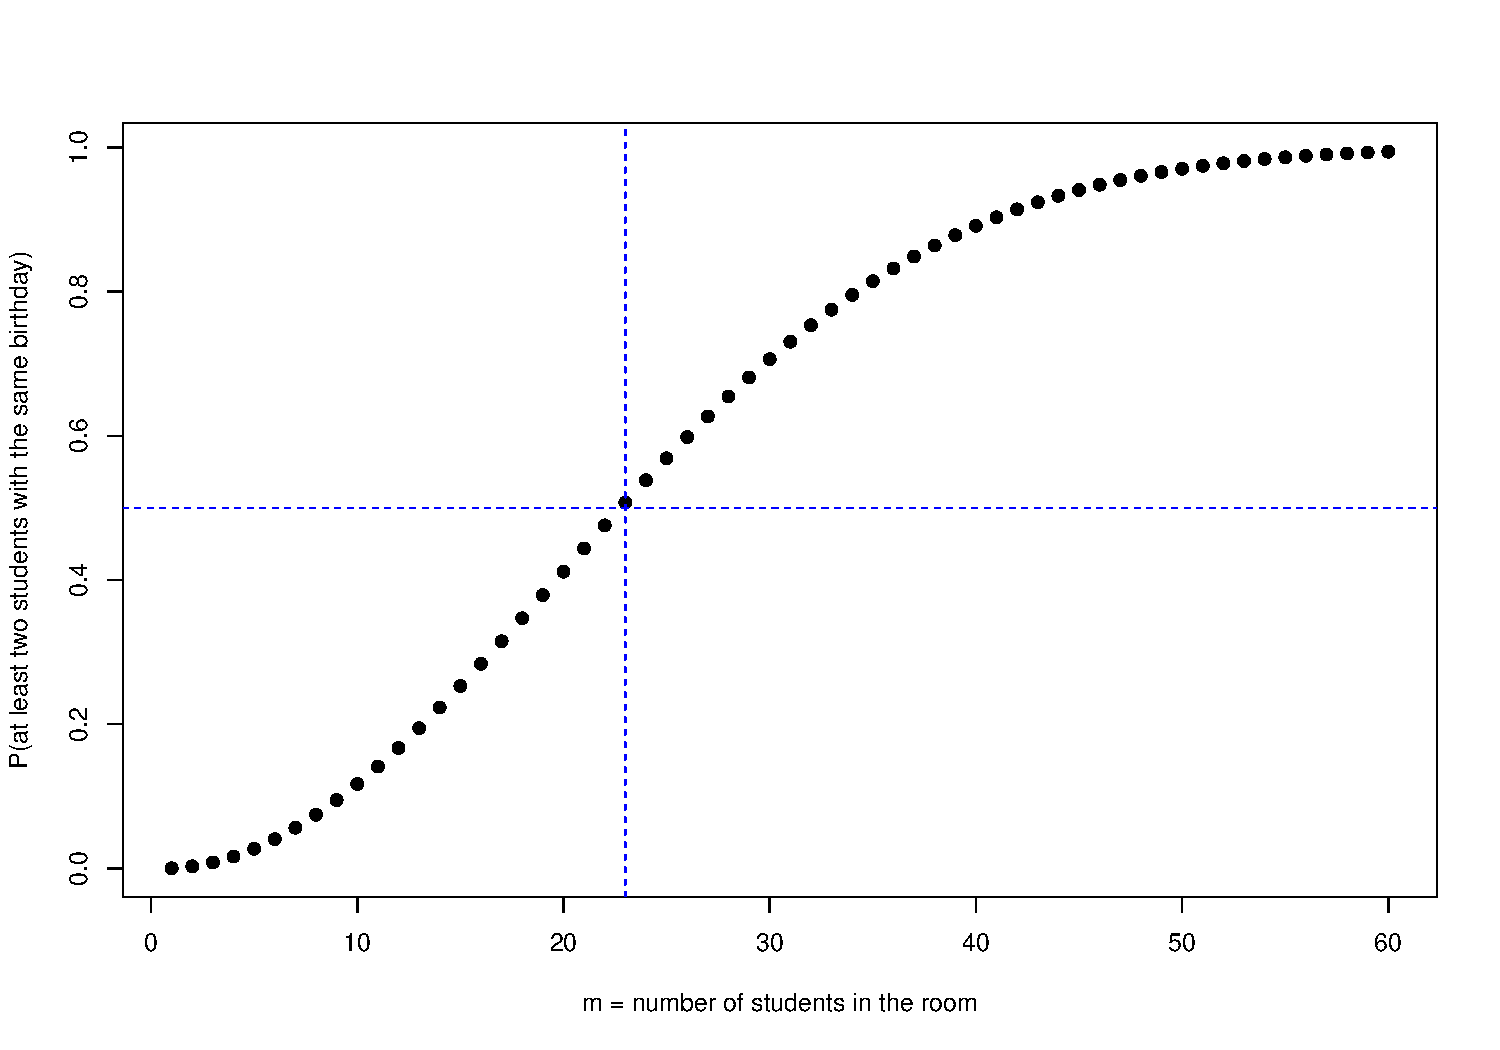
\includegraphics[width=0.3\linewidth,height=0.5\textheight]{Week7_Lect_files/figure-beamer/unnamed-chunk-1-1} \end{center}
\normalsize
\end{frame}

\begin{frame}{Addition Rules for Probability}
\protect\hypertarget{addition-rules-for-probability}{}
\begin{itemize}
\tightlist
\item
  If E and F can not happen happen at the same time (mutually exclusive
  or disjoint), then
  \[\textrm{\gilfont{P}}\normalfont (E \cup F)=\textrm{\gilfont{P}}\normalfont (E \text{ or } F) = \textrm{\gilfont{P}}\normalfont (E)+ \textrm{\gilfont{P}}\normalfont (F)\]
\end{itemize}

In general, for any sequence of mutually exclusive events
\(E_1, E_2, \ldots\) (that is \(E_i \cap E_j = \emptyset\)) for all
(\(i\neq j\))
\[\textrm{\gilfont{P}}\normalfont \left(\cup_{i=1}^{\infty} E_i\right)=\sum_{i=1}^{\infty} \textrm{\gilfont{P}}\normalfont (E_i)\]

\begin{itemize}
\tightlist
\item
  For any two events \(E\) and \(F\),
  \[\textrm{\gilfont{P}}\normalfont (E \cup F)=\textrm{\gilfont{P}}\normalfont (E \text{ or } F)=\textrm{\gilfont{P}}\normalfont (E)+ \textrm{\gilfont{P}}\normalfont (F)-\textrm{\gilfont{P}}\normalfont (E\cap F)\]
\end{itemize}
\end{frame}

\begin{frame}{Example 3}
\protect\hypertarget{example-3}{}
\begin{tcolorbox}
What is the probability of drawing a diamond or a spade from a standard card deck?
\end{tcolorbox}

\begin{tcolorbox}
Solution:

\vspace{30mm}
\end{tcolorbox}
\end{frame}

\begin{frame}{Example 4}
\protect\hypertarget{example-4}{}
\begin{tcolorbox}
What is the probability of drawing a diamond or an ace from a standard card deck?
\end{tcolorbox}

\begin{tcolorbox}
Solution:

\vspace{30mm}
\end{tcolorbox}
\end{frame}

\begin{frame}{Example 5}
\protect\hypertarget{example-5}{}
\begin{tcolorbox}
A class with 30 students consists of 16 Math majors, 21 CS majors and 8 double CS and Math majors. If a student is randomly selected, what is the probability that the student is a Math major or a CS major?
\end{tcolorbox}

\begin{tcolorbox}
Solution:

\vspace{30mm}
\end{tcolorbox}
\end{frame}

\begin{frame}{Multiplication Rules}
\protect\hypertarget{multiplication-rules}{}
\begin{itemize}
\tightlist
\item
  If \(E\) and \(F\) are independent
\end{itemize}

\[\textrm{\gilfont{P}}\normalfont (E \cap F) =\textrm{\gilfont{P}}\normalfont (E \text{ and } F)= \textrm{\gilfont{P}}\normalfont (E)\times \textrm{\gilfont{P}}\normalfont (F)\]
\end{frame}

\begin{frame}{Example 6}
\protect\hypertarget{example-6}{}
\begin{tcolorbox}
What is the probability of selecting 2 aces if 2 cards are randomly selected with replacement?
\end{tcolorbox}

\begin{tcolorbox}
Solution:


\vspace{30mm}


\end{tcolorbox}
\end{frame}

\begin{frame}{Conditional Probability and the General Multiplication
Rule}
\protect\hypertarget{conditional-probability-and-the-general-multiplication-rule}{}
\begin{itemize}
\tightlist
\item
  Another probability we want to be able to find is of the form ``given
  \(F\), what is the probability of \(E\)?'' This is known as a
  \textbf{conditional probability} and is written
\end{itemize}

\[\textrm{\gilfont{P}}\normalfont (E | F)=\frac{\textrm{\gilfont{P}}\normalfont ( E \cap  F)}{\textrm{\gilfont{P}}\normalfont ( F)}\]

\begin{itemize}
\tightlist
\item
  Rearranging the conditional probability equation, we get the
  \textbf{General Multiplication Rule}:
  \[\textrm{\gilfont{P}}\normalfont ( E \cap  F)=\textrm{\gilfont{P}}\normalfont ( F)\times \textrm{\gilfont{P}}\normalfont ( E| F)\]
\end{itemize}

Equivalently,
\[\textrm{\gilfont{P}}\normalfont (E \cap F)=\textrm{\gilfont{P}}\normalfont (E)\times \textrm{\gilfont{P}}\normalfont (F| E)\]
\end{frame}

\begin{frame}{Definition of Independence}
\protect\hypertarget{definition-of-independence}{}
\begin{itemize}
\tightlist
\item
  Events \(E\) and \(F\) are independent if knowing \(E\) happened does
  not change the probability of \(F\).
\end{itemize}

\[\textrm{\gilfont{P}}\normalfont ( E \cap  F)=\textrm{\gilfont{P}}\normalfont ( E)\times \textrm{\gilfont{P}}\normalfont ( F)\]
Then:
\[\textrm{\gilfont{P}}\normalfont ( E|  F)=\frac{\textrm{\gilfont{P}}\normalfont ( E \cap  F)}{\textrm{\gilfont{P}}\normalfont ( F)}=\frac{\textrm{\gilfont{P}}\normalfont ( E)\times \textrm{\gilfont{P}}\normalfont ( F)}{\textrm{\gilfont{P}}\normalfont ( F)}=\textrm{\gilfont{P}}\normalfont ( E)\]

\begin{itemize}
\item
  If \(E\) and \(F\) are independent then
  \(\textrm{\gilfont{P}}\normalfont ( E| F)=\textrm{\gilfont{P}}\normalfont ( E)\)
\item
  Equivalently
\end{itemize}

\[\textrm{\gilfont{P}}\normalfont (F|E)=\textrm{\gilfont{P}}\normalfont ( F)\]
\end{frame}

\begin{frame}{Example 7}
\protect\hypertarget{example-7}{}
\begin{tcolorbox}
What is the probability of selecting 2 aces if 2 cards are randomly selected without replacement?
\end{tcolorbox}

\begin{tcolorbox}
Solution:


\vspace{30mm}

\end{tcolorbox}
\end{frame}

\begin{frame}{Example 8}
\protect\hypertarget{example-8}{}
\begin{tcolorbox}
Suppose two fair dice are rolled where each of the 36 possible outcomes is equally likely to occur. Knowing that the first die shows a 3, what is the probability that the sum of the two dice equals 6?
\end{tcolorbox}

\begin{tcolorbox}
Solution: 

\vspace{30mm}


\end{tcolorbox}
\end{frame}

\hypertarget{law-of-total-probability-and-bayes-rule}{%
\section{Law of Total Probability and Bayes'
Rule}\label{law-of-total-probability-and-bayes-rule}}

\begin{frame}{Law of Total Probability and Bayes' Rule}
\protect\hypertarget{law-of-total-probability-and-bayes-rule-1}{}
\begin{itemize}
\item
  Bayes' Rule is used for reversing the condition

  \begin{itemize}
  \tightlist
  \item
    The formula is easier with the tree!
  \end{itemize}
\item
  In general: Let \(F_1, F_2, \ldots F_n\) be such that
  \(\cup_{i=1}^{\infty} F_i=\Omega\) and \(F_i\cap F_j=\emptyset\) for
  all \(i\neq j\), with \(\textrm{\gilfont{P}}\normalfont (F_i)>0\) for
  all \(i\). Then, for any event \(E\)
\end{itemize}

\[\textrm{\gilfont{P}}\normalfont (E)=\sum_{i=1}^n \textrm{\gilfont{P}}\normalfont (E \cap F_i)=\sum_{i=1}^n \textrm{\gilfont{P}}\normalfont (E|F_i)\textrm{\gilfont{P}}\normalfont (F_i)\]

\[\textrm{\gilfont{P}}\normalfont (F_i|E)=\frac{\textrm{\gilfont{P}}\normalfont (E \cap F_i)}{\textrm{\gilfont{P}}\normalfont (E)}=\frac{\textrm{\gilfont{P}}\normalfont (E|F_i)\textrm{\gilfont{P}}\normalfont (F_i)}{\sum_{i=1}^n\textrm{\gilfont{P}}\normalfont (E|F_i)\textrm{\gilfont{P}}\normalfont (F_i)}.\]
\end{frame}

\begin{frame}{Example 1}
\protect\hypertarget{example-1-1}{}
\begin{tcolorbox}
Suppose the prior probabilities that a document was written in Word, LaTeX, and HTML are: 0.50, 0.30, and 0.20, respectively.  From past experience it is known that 40\% of Word documents exceed 10 pages; 20\% of LaTeX documents exceed 10 pages; 20\% of HTML documents exceed 10 pages.  

\begin{itemize}
\item What is the overall proportion of documents containing more than 10 pages?
\item If the document that was chosen at random was found to exceed 10 pages, what is the probability it was written in LaTeX?
\item If the document that was chosen at random was found to exceed 10 pages, what is the probability it was written in Word?
\item If the document that was chosen at random was found to exceed 10 pages, what is the probability it was written in HTML?
\end{itemize}

\end{tcolorbox}
\end{frame}

\begin{frame}{Example 1 - Partial Solution}
\protect\hypertarget{example-1---partial-solution}{}
\begin{itemize}
\item Let $E$ be the event a document selected at random is more than 10 pages.
\item Let $W$ be the event the document is written with Word.
\item Let $L$ be the event the document is written with LaTeX.
\item Let $H$ be the event the document is written with HTML.
\end{itemize}

\[E = (W \cap E) + (L \cap E) + (H \cap E)\] \[
\begin{aligned}
\textrm{\gilfont{P}}\normalfont (E) &= \textrm{\gilfont{P}}\normalfont (W \cap E) + \textrm{\gilfont{P}}\normalfont (L \cap E) + \textrm{\gilfont{P}}\normalfont (H \cap E)\\
&= \textrm{\gilfont{P}}\normalfont (W)\textrm{\gilfont{P}}\normalfont (E|W) + \textrm{\gilfont{P}}\normalfont (L)P(E|L) + \textrm{\gilfont{P}}\normalfont (H)P(E|H)\\
&=(0.5 \times 0.4) + (0.30 \times 0.20) + (0.2 \times 0.2) = 0.30
\end{aligned}
\]

\begin{tcolorbox}
The probability a randomly selected document is more than 10 pages is 0.30.
\end{tcolorbox}
\end{frame}

\begin{frame}{Example 1 - Partial Solution}
\protect\hypertarget{example-1---partial-solution-1}{}
If the document that was chosen at random was found to exceed 10 pages,
what is the probability it was written in LaTeX? \[
\begin{aligned}
\textrm{\gilfont{P}}\normalfont (L | E) &= \frac{\textrm{\gilfont{P}}\normalfont (L)\cdot \textrm{\gilfont{P}}\normalfont (E|L)}{\textrm{\gilfont{P}}\normalfont (E)}\\
&=\frac{\textrm{\gilfont{P}}\normalfont (L)\cdot \textrm{\gilfont{P}}\normalfont (E|L)}{P(W \cap E) + \textrm{\gilfont{P}}\normalfont (L\cap E) + \textrm{\gilfont{P}}\normalfont (H \cap E)}\\
&=\frac{\textrm{\gilfont{P}}\normalfont (L)\cdot \textrm{\gilfont{P}}\normalfont (E|L)}{\textrm{\gilfont{P}}\normalfont (W)\textrm{\gilfont{P}}\normalfont (E|W) + \textrm{\gilfont{P}}\normalfont (L)\textrm{\gilfont{P}}\normalfont (E|L) + \textrm{\gilfont{P}}\normalfont (H)\textrm{\gilfont{P}}\normalfont (E|H)}\\
&=\frac{0.3 \times 0.2}{0.5 \times 0.4 + 0.3 \times 0.2 + 0.2 \times 0.2} \\
&=\frac{0.06}{0.3}= 0.2
\end{aligned}
\]

\begin{tcolorbox}
Given a randomly selected document was found to exceed 10 pages, the probability is was written in LaTeX is 0.2.
\end{tcolorbox}
\end{frame}

\begin{frame}{Example 1 - Partial Solution}
\protect\hypertarget{example-1---partial-solution-2}{}
If the document that was chosen at random was found to exceed 10 pages,
what is the probability it was written in Word? \[
\begin{aligned}
\textrm{\gilfont{P}}\normalfont (W | E) &= \frac{\textrm{\gilfont{P}}\normalfont (W)\cdot \textrm{\gilfont{P}}\normalfont (E|W)}{\textrm{\gilfont{P}}\normalfont (E)}\\
&=\frac{\textrm{\gilfont{P}}\normalfont (W)\cdot \textrm{\gilfont{P}}\normalfont (E|W)}{\textrm{\gilfont{P}}\normalfont (W \cap E) + \textrm{\gilfont{P}}\normalfont (L\cap E) + \textrm{\gilfont{P}}\normalfont (H \cap E)}\\
&=\frac{\textrm{\gilfont{P}}\normalfont (W)\cdot \textrm{\gilfont{P}}\normalfont (E|W)}{\textrm{\gilfont{P}}\normalfont (W)P(E|W) + \textrm{\gilfont{P}}\normalfont (L)\textrm{\gilfont{P}}\normalfont (E|L) + \textrm{\gilfont{P}}\normalfont (H)\textrm{\gilfont{P}}\normalfont (E|H)}\\
&=\frac{0.5 \times 0.4}{0.5 \times 0.4 + 0.3 \times 0.2 + 0.2 \times 0.2} \\
&=\frac{0.2}{0.3}= \frac{2}{3}
\end{aligned}
\]

\begin{tcolorbox}
Given a randomly selected document was found to exceed 10 pages, the probability is was written in Word is 2/3.
\end{tcolorbox}
\end{frame}

\begin{frame}{Example 1 - Partial Solution}
\protect\hypertarget{example-1---partial-solution-3}{}
If the document that was chosen at random was found to exceed 10 pages,
what is the probability it was written in HTML? \[
\begin{aligned}
\textrm{\gilfont{P}}\normalfont (H | E) &= \frac{\textrm{\gilfont{P}}\normalfont (H)\cdot \textrm{\gilfont{P}}\normalfont (E|H)}{\textrm{\gilfont{P}}\normalfont (E)}\\
&=\frac{\textrm{\gilfont{P}}\normalfont (H)\cdot \textrm{\gilfont{P}}\normalfont (E|H)}{\textrm{\gilfont{P}}\normalfont (W \cap E) + \textrm{\gilfont{P}}\normalfont (L\cap E) + \textrm{\gilfont{P}}\normalfont P(H \cap E)}\\
&=\frac{\textrm{\gilfont{P}}\normalfont (H)\cdot \textrm{\gilfont{P}}\normalfont (E|H)}{\textrm{\gilfont{P}}\normalfont (W)P(E|W) + \textrm{\gilfont{P}}\normalfont (L)\textrm{\gilfont{P}}\normalfont (E|L) + \textrm{\gilfont{P}}\normalfont (H)\textrm{\gilfont{P}}\normalfont (E|H)}\\
&=\frac{0.2 \times 0.2}{0.5 \times 0.4 + 0.3 \times 0.2 + 0.2 \times 0.2} \\
&=\frac{0.04}{0.3}= 0.1333333
\end{aligned}
\]

\begin{tcolorbox}
Given a randomly selected document was found to exceed 10 pages, the probability is was written in HTML is 0.1333333.
\end{tcolorbox}
\end{frame}

\begin{frame}{Example 2}
\protect\hypertarget{example-2}{}
\begin{tcolorbox}
Dan's Diner employs three dishwashers. Al washes $20\%$ of the dishes and breaks only $1\%$ of those he handles. Betty and Chuck each wash $40\%$ of the dishes, and Betty breaks only $1\%$ of hers, but Chuck breaks $5\%$ of the dishes he washes. You go to Dan's for supper one night and hear a dish break at the sink. What's the probability that Chuck is on the job?


\end{tcolorbox}
\end{frame}

\begin{frame}{Example 2}
\protect\hypertarget{example-2-1}{}
\begin{tcolorbox}
Solution:

\vspace{50mm}


\end{tcolorbox}
\end{frame}

\begin{frame}{Choose a Door}
\protect\hypertarget{choose-a-door}{}
\begin{tcolorbox}
The television show Let's Make a Deal hosted by Monty Hall, gave contestants the opportunity to choose one of three doors. Contestants hoped to choose the one that concealed the grand prize. Behind the other two doors were much less valuable prizes. After the contestant chose one of the doors, say Door 1, Monty opened one of the other two doors, say Door 3, containing a much less valuable prize. The contestant was then asked whether he or she wished to stay with the original choice (Door 1) or switch to the other closed door (Door 2). What should the contestant do? Is it better to stay with original choice of switch to the other closed door? (a) What is the probability of winning by switching doors when given the opportunity? (b) What is the probability of winning by staying with the initial selection?


\end{tcolorbox}
\end{frame}

\begin{frame}[fragile]{Choose a Door: \texttt{R} Code}
\protect\hypertarget{choose-a-door-r-code}{}
\small

\begin{Shaded}
\begin{Highlighting}[]
\FunctionTok{set.seed}\NormalTok{(}\DecValTok{13}\NormalTok{)}
\NormalTok{n }\OtherTok{\textless{}{-}} \DecValTok{10000}
\NormalTok{actual }\OtherTok{\textless{}{-}} \FunctionTok{sample}\NormalTok{(}\DecValTok{1}\SpecialCharTok{:}\DecValTok{3}\NormalTok{, }\AttributeTok{size =}\NormalTok{ n, }\AttributeTok{replace =} \ConstantTok{TRUE}\NormalTok{)}
\NormalTok{aguess }\OtherTok{\textless{}{-}} \FunctionTok{sample}\NormalTok{(}\DecValTok{1}\SpecialCharTok{:}\DecValTok{3}\NormalTok{, }\AttributeTok{size =}\NormalTok{ n, }\AttributeTok{replace =} \ConstantTok{TRUE}\NormalTok{)}
\NormalTok{equals }\OtherTok{\textless{}{-}}\NormalTok{ (actual }\SpecialCharTok{==}\NormalTok{ aguess)}
\NormalTok{not.eq }\OtherTok{\textless{}{-}}\NormalTok{ (actual }\SpecialCharTok{!=}\NormalTok{ aguess)}
\NormalTok{PnoSwitch }\OtherTok{\textless{}{-}} \FunctionTok{mean}\NormalTok{(equals)}
\NormalTok{PwiSwitch }\OtherTok{\textless{}{-}} \FunctionTok{mean}\NormalTok{(not.eq)}
\NormalTok{probs }\OtherTok{\textless{}{-}} \FunctionTok{c}\NormalTok{(PnoSwitch, PwiSwitch)}
\FunctionTok{names}\NormalTok{(probs) }\OtherTok{\textless{}{-}} \FunctionTok{c}\NormalTok{(}\StringTok{"P(Win no Switch)"}\NormalTok{, }\StringTok{"P(Win Switch)"}\NormalTok{)}
\NormalTok{probs}
\end{Highlighting}
\end{Shaded}

\begin{verbatim}
P(Win no Switch)    P(Win Switch) 
          0.3409           0.6591 
\end{verbatim}

\normalsize
\end{frame}

\begin{frame}{Choose a Door: Solution}
\protect\hypertarget{choose-a-door-solution}{}
To solve with Bayes' Rule, start by assuming the contestant initially
guesses Door 1 and that Monty opens Door 3. Let the event \(D_i=\) Door
\(i\) conceals the prize and \(O_j=\) Monty opens door \(j\) after the
contestant selects Door 1. When a contestant initially selects a door,
\(\textrm{\gilfont{P}}\normalfont (D_1)=\textrm{\gilfont{P}}\normalfont (D_2)=\textrm{\gilfont{P}}\normalfont (D_3)=1/3\).
(Similar reasoning works independent of the originally selected door.)
Once Monty shows the grand prize is not behind Door 3, the probability
of winning the grand prize is now one of
\(\textrm{\gilfont{P}}\normalfont (D_1|O_3)\) or
\(\textrm{\gilfont{P}}\normalfont (D_2|O_3)\). Note that
\(\textrm{\gilfont{P}}\normalfont (D_1|O_3)\) corresponds to the
strategy of sticking with the initial guess and
\(\textrm{\gilfont{P}}\normalfont (D_2|O_3)\) corresponds to the
strategy of switching doors. Based on how the show is designed, the
following are known:
\end{frame}

\begin{frame}{Choose a Door: Solution}
\protect\hypertarget{choose-a-door-solution-1}{}
\begin{itemize}
\item $\textrm{\gilfont{P}}\normalfont (O_3|D_1)=1/2$ since Monty can open one of either Door 3 or Door 2 without revealing the grand prize.
\item $\textrm{\gilfont{P}}\normalfont (O_3|D_2)=1$ since the only door Monty can open without revealing the grand prize is Door 3.
\item $\textrm{\gilfont{P}}\normalfont (O_3|D_3)=0$ since Monty will not open Door 3 if it contains the grand prize.
\end{itemize}
\end{frame}

\begin{frame}{Choose a Door: Solution}
\protect\hypertarget{choose-a-door-solution-2}{}
\begin{equation*}
\begin{split}
\textrm{\gilfont{P}}\normalfont (D_1|O_3)&=\dfrac{\textrm{\gilfont{P}}\normalfont (O_3|D_1)\textrm{\gilfont{P}}\normalfont (D_1)}{\textrm{\gilfont{P}}\normalfont (O_3|D_1)\textrm{\gilfont{P}}\normalfont (D_1)+\textrm{\gilfont{P}}\normalfont (O_3|D_2)\textrm{\gilfont{P}}\normalfont (D_2)+\textrm{\gilfont{P}}\normalfont (O_3|D_3)\textrm{\gilfont{P}}\normalfont (D_3)}\\
&=\dfrac{1/2 \times 1/3}{1/2 \times 1/3 + 1 \times 1/3 + 0 \times
1/3}=\dfrac{1}{3}.
\end{split}
\end{equation*}

\begin{equation*}
\begin{split}
\textrm{\gilfont{P}}\normalfont (D_2|O_3)&=\dfrac{\textrm{\gilfont{P}}\normalfont (O_3|D_2)\textrm{\gilfont{P}}\normalfont (D_2)}{\textrm{\gilfont{P}}\normalfont (O_3|D_1)\textrm{\gilfont{P}}\normalfont (D_1)+\textrm{\gilfont{P}}\normalfont (O_3|D_2)\textrm{\gilfont{P}}\normalfont (D_2)+\textrm{\gilfont{P}}\normalfont (O_3|D_3)\textrm{\gilfont{P}}\normalfont (D_3)}\\
&=\dfrac{1 \times 1/3}{1/2 \times 1/3 + 1 \times 1/3 + 0 \times
1/3}=\dfrac{2}{3}.
\end{split}
\end{equation*} Therefore, it is always to the contestant's benefit to
switch doors.
\end{frame}

\begin{frame}{Monte Hall Problem with \(n\) Doors}
\protect\hypertarget{monte-hall-problem-with-n-doors}{}
\begin{itemize}
\item
  Consider the case with \(n\) Doors and just one grand prize

  \begin{itemize}
  \tightlist
  \item
    The probability of winning the grand prize on the first choice is
    \(\frac{1}{n}\).
  \item
    This is the same probability of winning if you were to use the
    ``stay'' strategy.
  \end{itemize}
\item
  You will win the grand prize if both of the following events occur:

  \begin{itemize}
  \tightlist
  \item
    You choose a door that does not have the grand prize. Note:
    \(P(G)=\frac{n-1}{n}\).
  \item
    You choose the door with the grand prize by switching doors
    \(P(C|G)=\frac{1}{n-2}\).
  \end{itemize}
\end{itemize}
\end{frame}

\begin{frame}{Monte Hall Problem with \(n\) Doors}
\protect\hypertarget{monte-hall-problem-with-n-doors-1}{}
In other words, the probability of winning using the ``switch'' strategy
is
\[P(G \cap C)=P(G)\cdot P(C|G)=\frac{n-1}{n}\cdot \frac{1}{n-2}=\frac{n-1}{n(n-2)}\]
For \(n=3\) doors, the probability of winning with the ``switch''
strategy is: \[\frac{n-1}{n(n-2)}=\frac{3-1}{3(3-2)}=\frac{2}{3}\] Note:
\[\frac{n-1}{n(n-2)}> \frac{1}{n}\] This implies switching is always
better.
\end{frame}

\end{document}
